\documentclass[a4paper, 10pt]{article}


\usepackage[utf8]{inputenc}
\usepackage[a4paper, top=0.6in, right=0.8in, left=0.8in,bottom= 0.6in]{geometry}
% \usepackage{wrapfig, blindtext}
% \usepackage{graphicx}

%% packages

% \usepackage{blindtext} % needed for creating dummy text passages
%\usepackage{ngerman} % needed for German default language
\usepackage{amsmath} % needed for command eqref
\usepackage{amssymb} % needed for math fonts
\usepackage[
	colorlinks=true
	,breaklinks
	%,ngerman
	]{hyperref} % needed for creating hyperlinks in the document, the option colorlinks=true gets rid of the awful boxes, breaklinks breaks lonkg links (list of figures), and ngerman sets everything for german as default hyperlinks language
% \usepackage[hyphenbreaks]{breakurl} % ben�tigt f�r das Brechen von URLs in Literaturreferenzen, hyphenbreaks auch bei links, die �ber eine Seite gehen (mit hyphenation).
\usepackage{xcolor}
\definecolor{c1}{rgb}{0,0,1} % blue
\definecolor{c2}{rgb}{0,0.3,0.9} % light blue
\definecolor{c3}{rgb}{0.3,0,0.9} % red blue
\hypersetup{
    linkcolor={c1}, % internal links
    citecolor={c2}, % citations
    urlcolor={c3} % external links/urls
}
%\usepackage{cite} % needed for cite
\usepackage[round,authoryear]{natbib} % needed for cite and abbrvnat bibliography style
\usepackage[nottoc]{tocbibind} % needed for displaying bibliography and other in the table of contents
\usepackage{graphicx} % needed for \includegraphics 
\usepackage{longtable} % needed for long tables over pages
\usepackage{bigstrut} % needed for the command \bigstrut
\usepackage{enumerate} % needed for some options in enumerate
\usepackage{todonotes} % needed for todos
\usepackage{imakeidx} % needed for creating an index
\usepackage{fancyhdr}
\usepackage{float}

\pagestyle{fancy}
\fancyhf{}

\usepackage{bm}
\usepackage{tikz}
\usepackage{booktabs}
\usepackage{sectsty}
\usepackage{titlesec}

% ------------ Header/Footer hr ------------ %
\renewcommand{\headrulewidth}{0pt}
\renewcommand{\footrulewidth}{0.5pt}
\renewcommand{\arraystretch}{1,2}
% ------------ Header/Footer hr ------------ %

% ------------- Indentation ---------------- %
\setlength{\parindent}{0pt}
\setlength{\parskip}{10pt}
\setlength{\columnsep}{.5in}
% ------------- Indentation ---------------- %

% ------------------- subsubparagraph ------------------ %
\titleclass{\subsubparagraph}{straight}[\subparagraph]
\newcounter{subsubparagraph}
\renewcommand{\thesubsubparagraph}{\Alph{subsubparagraph}}
\titleformat{\subsubparagraph}[runin]{\normalfont\normalsize\bfseries}{\thesubsubparagraph}{1em}{}
\titlespacing*{\subsubparagraph} {\parindent}{3.25ex plus 1ex minus .2ex}{1em}
% ------------------- subsubparagraph ------------------ %

% ------------------- Table ------------------ %
\usepackage{array}
\usepackage{ragged2e}
\usepackage{microtype}
\newcolumntype{P}[1]{>{\raggedright\arraybackslash}p{#1}}
\newcolumntype{C}[1]{>{\centering\arraybackslash}p{#1}}
% ------------------- Table ------------------ %

% ------------------ Math -------------------------%
\thickmuskip=12mu plus 5mu minus 1mu            % Space after = sign
\medmuskip=8mu plus 2mu minus 3mu               % Space bt the Binary Operators
\thinmuskip=8mu          % Space after the Integral and comma, uniary Operators, I guess
% ------------------ Math -------------------------%

% ------------------ Section and Subsection -------------------------%
\titlespacing*{\section}{0pt}{*0.8}{*0.8}
\titlespacing*{\subsection}{0pt}{*0.8}{*0.8}
\titlespacing*{\subsubsection}{0pt}{*0.3}{*0.3}

\renewcommand{\thesection}{\Roman{section}} 
\renewcommand{\thesubsection}{\thesection.\Roman{subsection}}

\titleformat{\section}[block]{\large\bfseries\filcenter\hspace*{-0.5cm}\Roman{section}.}{}{1em}{}
\titleformat{\subsection}[block]{\bfseries\filcenter\hspace*{-0.5cm}\Roman{section}.\Roman{subsection}}{}{1em}{}
% ------------------ Section and Subsection -------------------------%

\usepackage{enumitem}
\usepackage{pdfpages}
% \setcounter{secnumdepth}{3}

\newcounter{tabrow}
\newcommand{\nextquestion}{\refstepcounter{tabrow}}

\numberwithin{equation}{section}

\title{{\Large\textbf{Google Summer of Code-2021}}}
\author{Devansh Shukla}
\date{}

\fancyfoot[c]{\thepage}
\fancyfoot[r]{devanshshukla99}

\newenvironment{focus}
    {   \hspace*{-0.2cm}
        \vspace*{-0.5cm}\begin{itemize}[label={$-$}]
        \setlength\itemsep{0.0cm}
    }
    {
        \end{itemize}\vspace*{-0.2cm}
    }

\newcommand{\pr}{
	{\color{blue} PR \#4591}
}

\begin{document}
	
	% \maketitle
	\begin{center}
		{\Large\textbf{Google Summer of Code - 2021}} \\
		\vspace*{0.4cm}
		{\large\textbf{Proposal for 3D Plotting in SunPy}} \\
		\vspace*{0.25cm}
		{\textbf{Devansh Shukla}} \\
		\vspace*{0.25cm}
		{\textbf{Mentors: Dr. David Stansby, Dr. Stuart Mumford and Dr. Nabil Freij}} 
		{\rule{\textwidth}{1pt}}
	\end{center}

	\section{Basic Information}
		\begin{tabular}{P{0.25\textwidth} P{0.7\textwidth}}
    \textbf{Name}: & Devansh Shukla \\
    \textbf{Pronouns}: & He/Him/His \\
    \textbf{Academic Program}: & Integrated Master of Science in Physics \\
    \textbf{Institution}: & Sardar Vallabhbhai National Institute of Technology, Surat, India (\href{https://www.svnit.ac.in}{svnit.ac.in}) \\
    \textbf{GitHub}: & \href{https://www.github.com/devanshshukla99}{@devanshshukla99} \\
    \textbf{Matrix}: & @devanshshukla99:matrix.org \\
    \textbf{E-Mail}: & \href{mailto:devanshshukla99@gmail.com}{devanshshukla99@gmail.com} \\
    \textbf{Contact No.}: & +91 9826887954 \\
    \textbf{Permanent Address}: & HNo. 269, Triveni Complex, One-Way Gate, Sagar, MP, India 470002 \\
    \textbf{TimeZone}: & IST | UTC +5:30 \\
\end{tabular}
	
	\section{Education Background}
		\begin{tabular}{P{0.25\textwidth} P{0.7\textwidth}}
    \textbf{Current Affiliation}: & Sardar Vallabhbhai National Institude of Technology, Surat, India. \\
    \textbf{Academic Program}: & Integrated Master of Science in Physics. \\
    \textbf{Expected Year of Graduation}: & 2023 \\
    & My Curriculum vitae -- \href{https://github.com/devanshshukla99/devanshshukla99/blob/ff7d9d9bbd5e70345af307bd22dce285b77fc72a/cv/cv_devanshshukla99.pdf}{CV} \\
\end{tabular}


	\section{Experience in Programming}
		\subsection{Software Skills}
    \begin{tabular}{P{0.25\textwidth} P{0.7\textwidth}}
        \textbf{Languages}: & Python, C \\
        \textbf{Platforms}: & Linux, Windows \\
        \textbf{Software \& Tools}: & \LaTeX, conda, WxMaxima, qspectrumanalyzer, 4nec2, GQRX, Mathematica. \\
    \end{tabular}
    \vspace*{-0.25cm}
\subsection{Open-Source Projects}
    % \begin{tabular}{P{.02\textwidth} P{.75\textwidth}}
    %     & $\bullet\quad$ \textbf{SAS-RFI}\\
    %     & \begin{focus}
    %         \item[$-$] Developed a Python program for Radio Frequency Interferance scan at Sardar Vallabhbhai National Institute of Technology, Surat, India.
    %         \item[$-$] \href{https://github.com/devanshshukla99/SAS}{github.com/devanshshukla99/SAS}
    %     \end{focus} \\
    %     & $\bullet\quad$ \textbf{Juno} \\
    %     & \begin{focus}
    %         \item[$-$] Developed a python program for straight-forward terminal-based socket communication with 128-bit AES encryption.
    %         \item[$-$] \href{https://github.com/devanshshukla99/Juno-ReDesign-Sockets-Communication/}{github.com/devanshshukla99/Juno-ReDesign-Sockets-Communication/}
    %     \end{focus} \\
    % \end{tabular}
    \begin{itemize}
        \item \textbf{SAS-RFI} \\
            \begin{focus}
                \item[$-$] Developed a Python program for Radio Frequency Interferance scan at Sardar Vallabhbhai National Institute of Technology, Surat, India.
                \item[$-$] \href{https://github.com/devanshshukla99/SAS}{github.com/devanshshukla99/SAS}
                \item[$-$] Analysed data and results at \href{https://github.com/devanshshukla99/Radio-Frequency-Interference-Scan}{github.com/devanshshukla99/Radio-Frequency-Interference-Scan}.
            \end{focus}
        \item \textbf{Juno} \\
            \begin{focus}
                \item[$-$] Developed a python program for straight-forward terminal-based socket communication with 128-bit AES encryption.
                \item[$-$] \href{https://github.com/devanshshukla99/Juno-ReDesign-Sockets-Communication/}{github.com/devanshshukla99/Juno-ReDesign-Sockets-Communication/}
            \end{focus}
        \item \textbf{Chromos} \\
            \begin{focus}
                \item[$-$] Package for getting colored text output in Python.
                \item[$-$] \href{https://github.com/devanshshukla99/Chromos}{github.com/devanshshukla99/Chromos}
            \end{focus}
    \end{itemize}


	\section{SunPy}
		\subsection{Why did I choose this Project: SunPy?}
    % I have been very interested in the AstroPhysics and Cosmology domain, but SunPy specifically caught my eye due to one of my course, \textit{Into. to Space Physics}, which included a seminar on Sun-spots in which I utilized SunPy to generate AIA and HMI Image of the Sun, thereby showing the correlation of sunspots and magnetic field;
    % I have been reading about SunPy since then, slowly learning about the awesome community.

    % This project brings out the best of both worlds, some Solar Physics and some Programming; for me it looked like a natural choice in my career to learn and hopefully contribute positively to the community.

    % More specifically, \autoref{sec:benefits_of_3d_plot} points to some benefits of 3D plotting I could see, ofcourse I'm open to find more in the future.

    % \todo[inline]{Find me a home!}
    % I will to contribute to SunPy even if I am not accepted, though I would prefer otherwise.

    % in this 3D plotting project if accepted, 

    I have been very interested in the Astrophysics and Cosmology domain for a long time. 
    SunPy specifically caught my eye due to my course, \textit{Intro. to Space Physics}, which included a seminar on Sun-spots in which I utilized SunPy to generate AIA and HMI Image of the Sun, thereby showing the correlation of sunspots and magnetic field; I have been reading about SunPy since then, slowly learning about the incredible community.
    
    I choosed this project since it brings out the best of both worlds, some Solar Physics and some Programming; for me, it looked like a natural choice in my career to learn and hopefully contribute positively to the community; more specifically,  \autoref{sec:benefits_of_3d_plot} points to some reasons and benefits of such a project; of course, I'm open to finding more in the future.
		\subsection{Benefits of 3D Plotting} \label{sec:benefits_of_3d_plot}
    \begin{focus}
        \item Super useful when combining visualizations of multiple objects, for example combining HMI with AIA Image or adding a LASCO Map.
        \item Good for intuitive understanding.
        \item For Example, PFSSPy, a dependent of SunPy, has a feature of overplotting field lines over an AIA Map, such a feature would be benefitted a lot if there is 3D plot support in SunPy. (\autoref{fig:pfsspy}).
        \item Looks super cool.
    \end{focus}
    \begin{figure}[H]
        \centering
        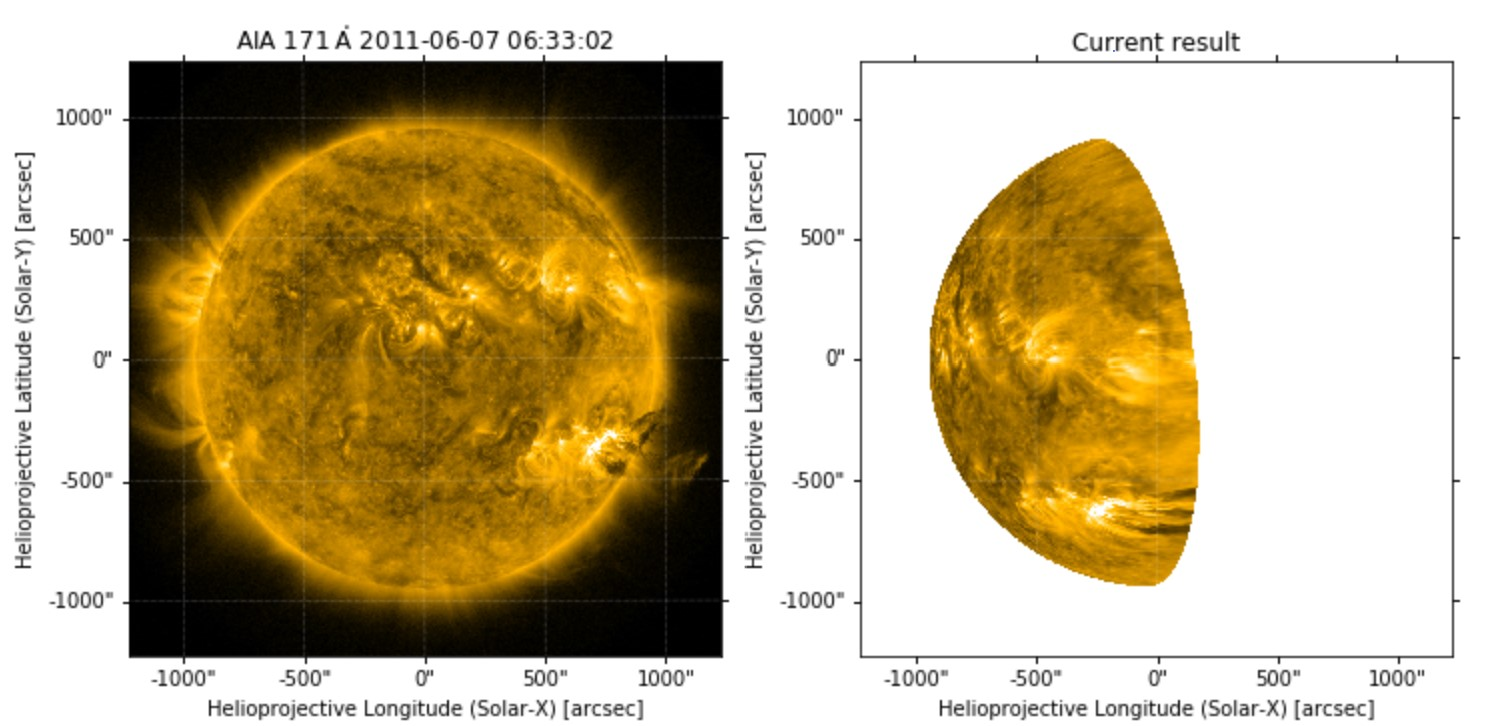
\includegraphics[scale=0.5]{figs/fig_3d_1.jpg}
        \caption{Example for show-casing usefulness of 3D plots, Issue \# 3997}
        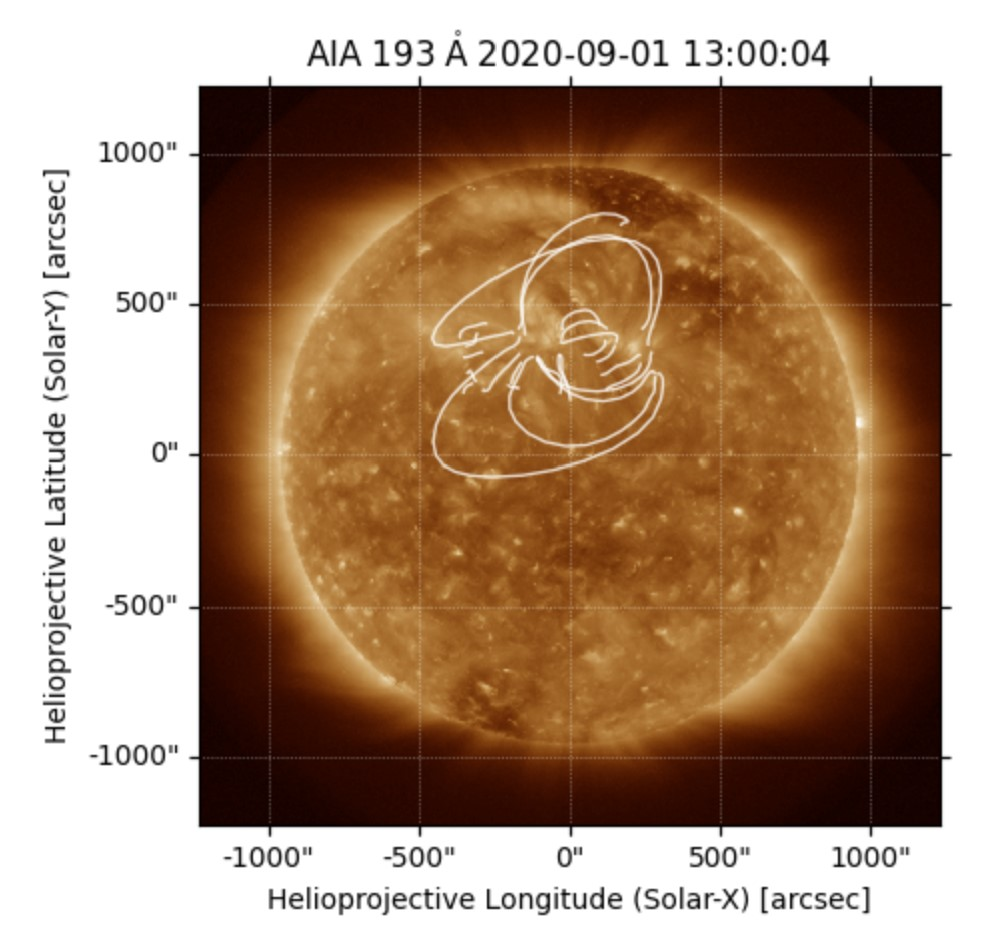
\includegraphics[scale=0.5]{figs/fig_3d_pfss_2.jpg}
        \caption{Overplotting field lines over an AIA Map with PFSSPy}
        \label{fig:pfsspy}
    \end{figure}

		\subsection{What have other people contributed to this project previously?}
    Presently, \pr by Dr. David Stansby(@dstansby) provides a foundation for the project. It's basically a proof-of-concept; it takes a sunpy.map.Map object, converts it to Heliocentric-Inertial Coordinate system, creates a mesh and finally plots in PyVista.
    

		\subsection{My Contributions}
    \textbf{PR \#5193}: Under Review
    \begin{focus}
        \item Adds support for file-handlers and file-type in Map and TimeSeries.
        \item \href{https://github.com/sunpy/sunpy/pull/5193}{github.com/sunpy/sunpy/pull/5193}
    \end{focus}
    \textbf{Issue \#3303}: Currently working
        \begin{focus}
            \item Create a Test or a function to report status on all remote servers SunPy pings during a test run.
            \item Thinking about using a pytest plugin to intercept the requests with a flag but it likly to change. :)
            \item \href{https://github.com/sunpy/sunpy/issues/3303}{github.com/sunpy/sunpy/issues/3303}
        \end{focus}


	\section{Project: 3D Plotting in SunPy}
		\subsection{Project Abstract}
SunPy currently uses Matplotlib for plots and has no support for 3D plots except PR\#4591.

		% \subsection{Copied Milestones}
    \begin{itemize}
        \item Put code for plotting 3D maps into a new Python package
        \item Add documentation and tests
        \item Add code for plotting astropy coordinate objects
        \item If time permits, add extra 3D plotting functionality (there’s plenty of data types we could tackle!)
    \end{itemize}
		\subsubsection{Goals}
    % The goal of the project is to throw \pr into a new package and develop an API intially using pyvista but general enough for other backends like plotly.
    % \begin{itemize}
    %     \item Convert code from \pr into a new package under SunPy org.
    %     \item Hoping for 90\%, targeting 100\% code-coverage.
    %     \item Add documentation.
    %     \item Add infrastructure to plot astropy coordinate object.
    %     \item Add infrastructure to support other data types too.
    % \end{itemize}

\begin{itemize}
    \item Convert code from \pr into a new package under SunPy org, and understand it down it a fiber.
    \item Add infrastructure to plot astropy coordinate object.
    \item Add infrastructure to support other data types, too, like for SOHO, RHESSI, etc.
    \item Hoping for 90\%, targeting 100\% code-coverage. Benchmarks and extra optimizations, if possible.
    \item Complete documentation
\end{itemize}

In all, we have to prepare a pre-release of the package for 3D support.

		\subsection{Time Commitment}
    I plan to commit and immerse fully into the project, with a minimum investment of 20hr/week to a maximum of 35hr/week and an average of 30hr/week.
    Honestly, I am not a big fan of assesing based on time-investment, my first priority would be to make and follow weekly task schedules, with some buffer time for unforeseeable circumstances and additional tests. 

		\subsection{Timeline}
    % Attached a thorough  timeline of the proposed project.
    % Regarding my commitments, I will have my college from August 10, so I've shifted some of my workload to July.

    % I am also eager to publish a weekly blog for the project with all relevent details to help future developers and people using 3D plotting in SunPy.
    I have attached a thorough timeline of the proposed project. 
    Regarding my commitments, I'll have my course classes from August 10, so I've shifted some of the workload to July.
    
    I am super eager to publish a weekly blog for the project with all relevant details to help future developers and users; I believe this would be critical in the long run.
   
    \begin{itemize}
        \item \textbf{May 17, 2021 - May 24, 2021} \\
            \begin{focus}
                \item Familiarize with the code and the community.
                \item Since I am already familiar with the dev env and test systems used in SunPy(tox, pytest) I'll focus more on the code and how it all is integrated together.
                \item Create a separate package with \pr as foundation and set-up all necessary workflows.
            \end{focus}
        \item \textbf{May 24, 2021 - June 1, 2021} \\
            \begin{focus}
                \item During this time, I'll discuss with my mentors and come with more specific details about the project, like how the public face of the API should behave, etc.
                \item I'll learn and try to solve the challenges I'm already aware-of in the project, see autoref%\autoref{sec:issues_identified}
                \item Dependencies like AstroPy, plotly, MPL, PyVista.
            \end{focus}
            \item \textbf{May 24, 2021 - June 1, 2021} \\
            \begin{focus}
                \item Plan for the API.
                \item Throughly understand and test the existing code.
                \item Dependencies like AstroPy, plotly, MPL, PyVista.
            \end{focus}
        \item \textbf{June 7, 2021 - June 14, 2021} \\
            \begin{focus}
                \item Define tests and documentation for the existing code.
                \item Discuss \& Work on the API.
            \end{focus}
        \item \textbf{June 14, 2021 - June 21, 2021} \\
            \begin{focus}
                \item Add code for plotting sunpy.map.Map
                \item Work on the API.
                \item Crush the bugs along the way.
            \end{focus}
        \item \textbf{June 21, 2021 - June 28, 2021} \\
            \begin{focus}
                \item Add tests and documentation, hoping to achieve 75\%+ code coverage.
                \item Check the Integration with SunPy. -- Waypoint - 1 Check
            \end{focus}
        \item \textbf{June 21, 2021 - June 28, 2021} \\
            \begin{focus}
                \item Crush the bugs.
                \item Add tests and documentation, hoping to achieve 90\%+ targeting 100\% code coverage.
                \item Finalizing the API.
            \end{focus}
        \item \textbf{June 28, 2021 - July 5, 2021} \\
            \begin{focus}
                \item Gather Feedback.
                \item Finalizing the API for the evaluation.
                \item Crush the Bugs.
            \end{focus}
        \item \textbf{July 5, 2021 - July 12, 2021} \\
            \begin{focus}
                \item Finalizing the API for the evaluation.
                \item Plan for plotting astropy coordinates in 3D infrastructure.
                \item Buffer time.
            \end{focus}
        \item \textbf{July 12, 2021 - July 16, 2021} \\
            \begin{focus}
                \item Buffer time, for incorporating required changes as per feedback.
                \item More debugging.
            \end{focus}
        \item \textbf{June 16, 2021 - July 23, 2021} \\
            \begin{focus}
                \item Work on infrastructure for plotting astropy coordinates in 3D.
                \item Discuss on adding infrastructure for other data type.
            \end{focus}
        \item \textbf{July 23, 2021 - July 30, 2021} \\
            \begin{focus}
                \item Test infrastructure for plotting astropy coordinates in 3D.
                \item Plan infrastructure for other data type, SOHO, EUV, RHEISSI, tbd.
                \item Buffer time to crush bugs.
            \end{focus}
        \item \textbf{July 30, 2021 - August 6, 2021} \\
            \begin{focus}
                \item Work on adding infrastructure for other data type, SOHO, EUV etc, tbd.
                \item Add tests and documentations, hoping to achieve 75\%+.
            \end{focus}
        \item \textbf{August 6, 2021 - August 13, 2021} \\
            \begin{focus}
                \item Work on support of pyvista for jupyter-notebook.
                \item Crush the bugs.
                \item Finalize the API.
            \end{focus}
        \item \textbf{August 13, 2021 - August 20, 2021} \\
            \begin{focus}
                \item Add tests and documentations, hoping to achieve 90\%+ targeting 100\% code coverage.
                \item Finalize the API, prepare for the pre-release.
                \item Crush the bugs.
                \item Check Documentation for mistakes/typos/bugs.
            \end{focus}
        \item \textbf{August 13, 2021 - August 16, 2021} \\
            \begin{focus}
                \item Finalize the API, incorporate the feedback from additional review.
                \item Crush the bugs.
                \item Gather feedback.
            \end{focus}
        \item \textbf{August 16, 2021 - August 23, 2021} \\
            \begin{focus}
                \item Pre-Release. 
                \item Crush the Bugs.
            \end{focus}
        \item \textbf{August 23, 2021 - } \\
            \begin{focus}
                \item Maintain support and work on improving the performance and stuff.
                \item Keep crushing the bugs.
            \end{focus}
    \end{itemize}
		\subsection{Probable Issues/Challenges:} \label{subsec:issues_challenges}
    \vspace*{-0.5cm}
    \begin{focus}
        \item The API will initially depend upon pyvista, which works on VTK, unfortunately Read the Docs doesn't support a headless-display, but this need to be investigated after reply from @cadair \href{https://github.com/sunpy/sunpy/pull/4591#issuecomment-749542653}{suggesting a possible solution}.
        \item As of now, whenever I run pyvista from Jupyter Notebook it bugs out crashing the notebook, I'm not sure if this is a wide-spread or localised issue.
    \end{focus}
			
	\section{GSoC}
		      
\paragraph*{Have you participated previously in GSoC? \\} \vspace*{-0.2cm}
    \vspace*{0.1cm}
    This is the first time I'm applying to a project.
\paragraph*{Are you also applying to other projects? \\} \vspace*{-0.2cm}
    \vspace*{0.1cm}
    This is the only proposal I'm submitting.
\paragraph*{How much time do you to invest in the project before, during and after Summer of Code? \\} \vspace*{-0.2cm}
    \vspace*{0.1cm}
    \begin{focus}
        \item Before - 20hrs/week.
        \item During - 25hrs/week.
        \item After - 15hrs/week.
    \end{focus}

\paragraph*{Are you eligible to receive payments from Google? \\} \vspace*{-0.2cm}
    \vspace*{0.1cm}
    Yes, I am eligible.

	
\end{document}